\originalchapter{作业十：同粒子、吸附与熵最大化}
\psource{8.044，2013 春，PS10，5 月 3 日截止。中文题面；据官方答案核对的 AI 独立解答。}
\originalsection{1．三个单粒子态中的两粒子}
\begin{exercise}
两个相同、无自旋、非相互作用粒子，单粒子态 $\psi_1,\psi_2,\psi_3$，能量 $0<\epsilon_2<\epsilon_3$（$\epsilon_1=0$）。
(a) 用占据数逐行列全部费米两体态及能量，标出零温态；(b) 对玻色重复；(c) 写两种固定粒子数正则 $Z$；(d) 各保留最低两个能量项求内能温度依赖，比较零温行为。
\end{exercise}
\begin{solution}
(a) 费米态为 $(1,1,0):\epsilon_2$（基态），$(1,0,1):\epsilon_3$，$(0,1,1):\epsilon_2+\epsilon_3$。
(b) 玻色态为 $(2,0,0):0$（基态），$(1,1,0):\epsilon_2$，$(1,0,1):\epsilon_3$，$(0,2,0):2\epsilon_2$，$(0,1,1):\epsilon_2+\epsilon_3$，$(0,0,2):2\epsilon_3$；其中中间两项的次序依 $\epsilon_3$ 与 $2\epsilon_2$ 而定。
(c) $Z_F=e^{-\beta\epsilon_2}+e^{-\beta\epsilon_3}+e^{-\beta(\epsilon_2+\epsilon_3)}$，$Z_B=1+e^{-\beta\epsilon_2}+e^{-\beta\epsilon_3}+e^{-2\beta\epsilon_2}+e^{-\beta(\epsilon_2+\epsilon_3)}+e^{-2\beta\epsilon_3}$。
(d) 令 $\delta=\epsilon_3-\epsilon_2$，$U_F\simeq\epsilon_2+\delta/(e^{\beta\delta}+1)$，$U_B\simeq\epsilon_2/(e^{\beta\epsilon_2}+1)$。最低温分别为 $\epsilon_2+\delta e^{-\beta\delta}$ 与 $\epsilon_2e^{-\beta\epsilon_2}$；基能与激发间隙均不同。这些分母来自两体态截断，不是误将粒子统计换成费米统计。
\end{solution}
\originalsection{2．两单粒子态的玻色系统}
\begin{exercise}
$N$ 个无自旋理想玻色粒子只有能量 $0,\Delta>0$ 的两个单粒子态。(a) 用占据数标记全部多体态、能量与态数；(b) 求闭式 $Z(N,T)$；(c) 求上态有 $n$ 粒子的概率；(d) 同样单粒子态但粒子可区分时的 $Z_d$。
\end{exercise}
\begin{solution}
态为 $(N-n,n)$，$n=0,\ldots,N$，$E_n=n\Delta$，共 $N+1$ 态。$q=e^{-\beta\Delta}$，$Z=(1-q^{N+1})/(1-q)$，$p(n)=(1-q)q^n/(1-q^{N+1})$。高温 $q\to1$ 时为 $1/(N+1)$。可区分时 $Z_d=(1+q)^N$，每个总占据数有 $\binom Nn$ 种不同微态，不能遗漏此简并。
\end{solution}
\originalsection{3．氯分子的 Raman 交替线}
\begin{exercise}
先用本书同粒子交换与 Raman 章节代替原题指定的官方 notes 阅读。氯的稳定同位素 $^{35}$Cl、$^{37}$Cl 的原题比例 76\%、24\%，核自旋均 $3/2$。
(a) 纯 $^{35}$Cl$_2$ 转动 Raman 两组交替线强度包络之比；(b) 包络因子 $(2L+1)e^{-L(L+1)\Theta_R/T}$ 在哪一 $L$ 附近最大；(c) $\Theta_R(\mathrm N_2)=2.9$ K，与 notes 的室温谱比较；氯 $\Theta_R=.35$ K，估计峰前线数；(d) 若只有 $^{35}$Cl--$^{37}$Cl 异核分子，谱怎样改变？
\end{exercise}
\begin{solution}
(a) 两个自旋 $3/2$ 核为费米子。对称核自旋态数 $7+3=10$，反对称 $5+1=6$；偶 $L$ 的空间对称配反对称自旋，奇 $L$ 相反，所以偶:奇包络 $6:10=3:5$。这一比值是在去除缓变 Boltzmann、转动简并及散射矩阵元之后的交替权重。
(b) 连续求导给 $(2L+1)^2=2T/\Theta_R$，$L_*=[\sqrt{2T/\Theta_R}-1]/2$，常粗略取 $\sqrt{T/(2\Theta_R)}$。
(c) 取原 notes 室温约 300 K。上述 $L_*$ 只定位未乘核自旋权重的连续包络；最强离散线还要比较
\[I_L\propto g_L(2L+1)e^{-L(L+1)\Theta_R/T},\]
这里沿原 notes 用转动能级占据数估计线强，省略共同归一化因子和散射矩阵元变化。$^{14}$N 核自旋为1、属玻色子，偶/奇 $L$ 的核自旋权重 $g_L$ 分别为6/3。氮的包络峰 $L_*\simeq6.69$，实际加权比较 $I_6\simeq51.9722$、$I_7\simeq26.1887$、$I_8\simeq50.8547$，最强为偶支 $L=6$。从 $L=0\to2$ 的第一条 Stokes 线起计，是\textbf{第7条}。官方解用未加权包络的 $L\simeq7$ 说氮谱最强在第8条，遗漏了交替权重；包络位置与最强单线须区分。

氯的包络峰 $L_*\simeq20.20$，偶/奇权重为6/10；强奇支的候选 $L=19,21$ 中，$I_{19}\simeq250.3384$、$I_{21}\simeq250.8325$，而偶支峰 $I_{20}\simeq150.7061$，所以最强为 $L=21$，同样计数是\textbf{第22条}。各支的包络在 $L_*$ 前增、后减，故只须比较峰两侧同奇偶的邻近整数；脚本实际枚举亦确认结果。这里不计未发生频移的Rayleigh中心线，也不把反Stokes线另加进序数。氯的第22条与官方估计相同，但必须由加权离散比较解释，不能从 $20.20$ 直接说第21条最强。
(d) 两核可区分，无交换筛选，所有转动态有共同核自旋权重 16，交替强弱消失；转动惯量变化还会略改线距。
\end{solution}
\originalsection{4．Langmuir 等温线}
\begin{exercise}
$M\ge N$ 个不同位点，每处最多一个相同原子，每个吸附能 $-\epsilon_0$。
(a) 放置方法数；(b) 固定 $N$ 正则 $Z$；(c) 求 $F$ 和大体系 $\mu=-\epsilon_0-\kb T\ln[(M-N)/N]$；(d) 与三维经典同种气体密度 $n$、热波长 $\lambda_T$ 平衡，求位点占据 $f=N/M$，形式上令 $h\to0$ 会怎样；(e) 用气压 $P$ 表示并画恒温等温线。
\end{exercise}
\begin{solution}
(a) $\Omega=\binom MN$；(b) $Z=\binom MN e^{\beta N\epsilon_0}$；(c) $F=-N\epsilon_0-\kb T\ln\binom MN$，用 Stirling 并求 $N$ 导数得所求化学势，边界用离散自由能差。
(d) $\mu_g=\kb T\ln(n\lambda_T^3)$，相等得 $f=x/(1+x)$，$x=n\lambda_T^3e^{\beta\epsilon_0}$。在固定其他模型参数的形式极限 $h\to0$，$\lambda_T\to0,f\to0$；真实绑定能、谱亦源于量子力学，不能由此断言物理世界可连续保持相同吸附模型。
(e) $f=KP/(1+KP)$，$K=\lambda_T^3e^{\beta\epsilon_0}/(\kb T)$，初始斜率 $K$，高压趋 1。
\end{solution}
\begin{center}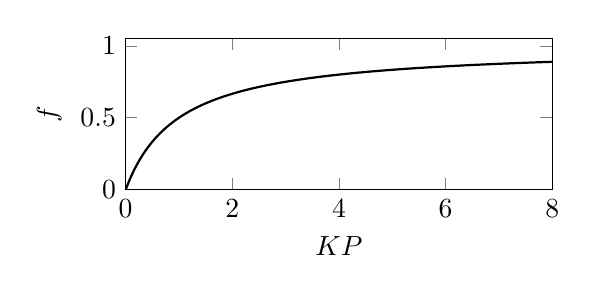
\begin{tikzpicture}\begin{axis}[width=7cm,height=3.5cm,xmin=0,xmax=8,ymin=0,ymax=1.05,xlabel={$KP$},ylabel={$f$},samples=100]\addplot[domain=0:8,thick]{x/(1+x)};\end{axis}\end{tikzpicture}\end{center}
\originalsection{5．信息熵到巨正则概率}
\begin{exercise}
原题参考 Blundell \& Blundell 第 15.1 节和附录 C.13；这里保留阅读引用并完整给出 MIT 问题。信息量为 $-\ln p$，平均信息熵假设等于 $S_I=-\kb\sum_i p_i\ln p_i$。
(a) 等概率微正则 $p=1/\Omega$ 检验热熵；(b) 正则 $p_i=e^{-\beta E_i}/Z$、$F=-\kb T\ln Z$ 检验；(c) 巨正则态标记 $(N,\nu)$，在 $\sum p=1,\sum Ep=U,\sum Np=\bar N$ 下最大化熵，用拉格朗日乘子证明 $\ln p=\lambda_1/\kb-1+(\lambda_U/\kb)E+(\lambda_N/\kb)N$；(d) 乘 $\kb p$ 求和与 $\Phi=U-TS-\mu\bar N$ 比较，确定乘子并得标准概率。
\end{exercise}
\begin{solution}
(a) $S_I=\kb\ln\Omega$。(b) $S_I=\kb\beta U+\kb\ln Z=(U-F)/T$。
(c) 取 $L=S_I+\lambda_1\sum p+\lambda_U\sum Ep+\lambda_N\sum Np$，固定约束常数可略；对每概率求导，$-\kb(\ln p+1)+\lambda_1+\lambda_UE+\lambda_NN=0$。熵严格凹，归一化分布存在时此驻点为最大而非最小。
(d) 求和先得 $-S=(\lambda_1-\kb)+\lambda_UU+\lambda_N\bar N$，但这一标量式本身不足以分别确定三个乘子。固定 $V$ 及微观能谱，沿最优概率分布改变 $U,\bar N$；由 (c) 的驻点式和归一化 $\sum_i\dd p_i=0$，
\[\dd S=-\kb\sum_i(\ln p_i+1)\dd p_i
=-\lambda_U\sum_iE_i\dd p_i-\lambda_N\sum_iN_i\dd p_i
=-\lambda_U\dd U-\lambda_N\dd\bar N.\]
热力学在固定 $V$ 时给 $\dd S=\dd U/T-\mu\dd\bar N/T$；两个约束量可局部独立改变，故 $\lambda_U=-1/T$、$\lambda_N=\mu/T$。于是令 $\Xi=\sum_i e^{\beta(\mu N_i-E_i)}$，归一化要求 $e^{\lambda_1/\kb-1}\Xi=1$，给
\[\lambda_1-\kb=-\kb\ln\Xi,\qquad
p_{N\nu}=\frac{e^{\beta(\mu N-E_{N\nu})}}\Xi.\]
再代回求和式，与 $\Phi=U-TS-\mu\bar N$ 一致地得到 $\lambda_1-\kb=\Phi/T$、$\Phi=-\kb T\ln\Xi$。这些关系以归一化和有限平均量存在为前提。原题把单条信息内容写成 $\ln P_i$，正信息量应为负号。
\end{solution}
\originalsection{6．含化学势的 Maxwell 关系}
\begin{exercise}
用不含化学势的其他偏导表示 $(\partial S/\partial\mu)_{V,N}$、$(\partial\mu/\partial V)_{T,N}$、$(\partial\mu/\partial P)_{T,N}$、$(\partial\mu/\partial T)_{P,N}$。
\end{exercise}
\begin{solution}
依次由 $U(S,V,N),F(T,V,N),G(T,P,N)$ 的混合偏导得
\begin{align*}
S_\mu|_{V,N}&=N_T|_{S,V},&\mu_V|_{T,N}&=-P_N|_{T,V},\\
\mu_P|_{T,N}&=V_N|_{T,P},&\mu_T|_{P,N}&=-S_N|_{T,P}.
\end{align*}
第一式需相关映射局部可逆。第三式必须保持题给 $T$；官方答案末尾从焓推导的是固定 $S$ 的另一关系，不能替代此题要求。
\end{solution}
